In this part of the system, a feature set used for unary potential is more diverse than previously, as it contains contextual data about image superpixels. In the already mentioned article by Jamie Shotton \cite{article_main}, the key component of the unary potential is a texture-layout potential, which operates on a texton map, and not on the original image. Therefore, before the segmentation process can take place a classification into textons needs to be conducted. Then, each pixel is assigned to exactly one texton, which makes it possible to model the relations between textures of neighbouring pixels. However, the dataset generated for the experiments described in this chapter do not contain any texture information and the only difference between objects is their colours and shapes. Hence, instead of performing a process of textonisation, colour quantisation was introduced. Then, each assignment of the pixel to a given colour from the reduced colour palette simulates the assignment to a single texton. As images from the generated dataset are composed of regions in the shades of red, green, and blue, after the quantisation process tricoloured images are obtained, which are similar to the ones presented in the first experiment of the previous chapter. Those generated images are presented in Figure \ref{fig:nonlinear_quantisation}.
\begin{figure}[ht]
    \centering
    \begin{tabular}{ccc}
        \fcolorbox{black}{white}{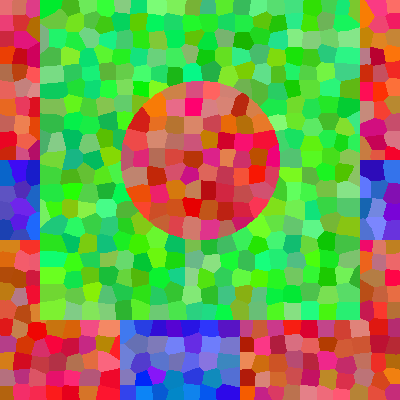
\includegraphics[width = 0.28\textwidth]{nonlinear_intro/circle.png}} &
        \fcolorbox{black}{white}{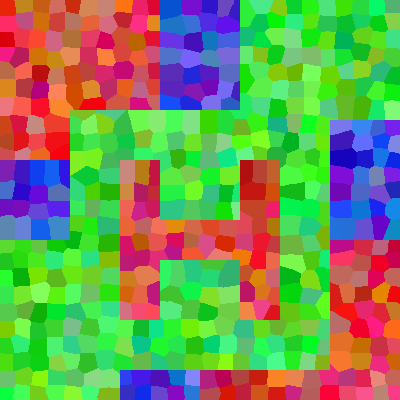
\includegraphics[width = 0.28\textwidth]{nonlinear_intro/letter_h.png}} &
        \fcolorbox{black}{white}{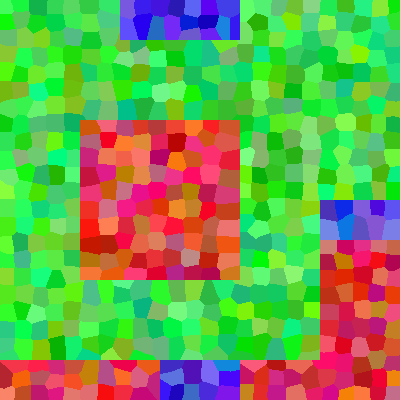
\includegraphics[width = 0.28\textwidth]{nonlinear_intro/square.png}} 
        \\
        \fcolorbox{black}{white}{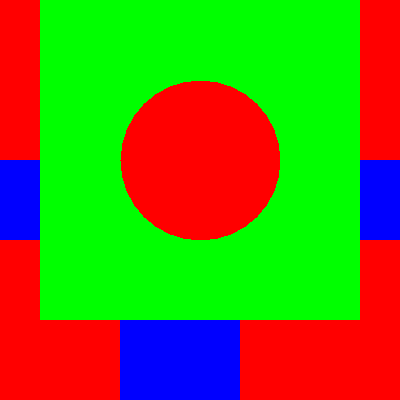
\includegraphics[width = 0.28\textwidth]{nonlinear_intro/circle_quant.png}} &
        \fcolorbox{black}{white}{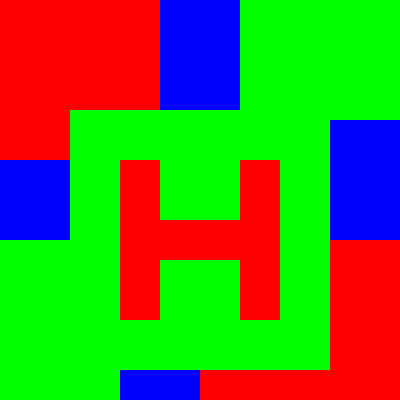
\includegraphics[width = 0.28\textwidth]{nonlinear_intro/letter_h_quant.png}} &
        \fcolorbox{black}{white}{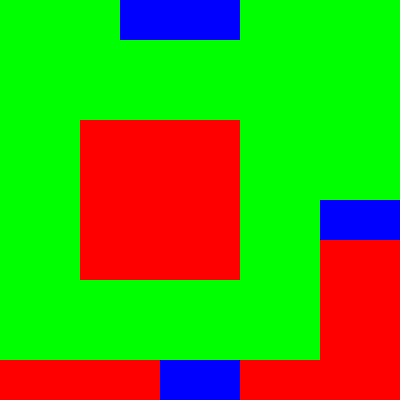
\includegraphics[width = 0.28\textwidth]{nonlinear_intro/square_quant.png}} 
    \end{tabular}
    \caption{Sample images after the process of colour quantisation.}
    \label{fig:nonlinear_quantisation}
\end{figure}

Having the dataset transformed into colour maps there is a need to extract features that are going to be used to compute the aimed unary potential. For the task of shape differentiation, two types of features were introduced and both of them include contextual data. The very first step that is needed obtain such features is to define a boundary of influence for a given superpixel. It was achieved by creating a regular grid of points around the centre of mass of the chosen superpixel. The distance between grid points is defined as a mean distance between neighbouring superpixel centres in the whole image, and the size of a created grid is a hyperparameter that should be fixed before feature extraction takes place. Then, each point in a resulting grid represents exactly one neighbour which have an influence on a given superpixel during the energy computations.
\begin{figure}[ht]
    \centering
    \begin{subfigure}[h]{0.40\textwidth}
        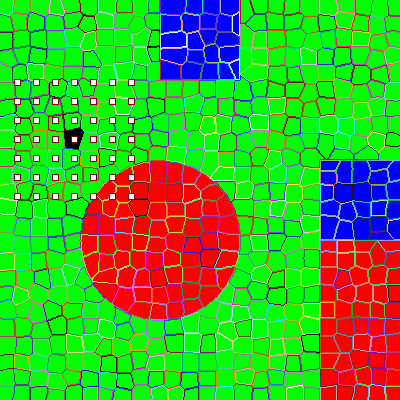
\includegraphics[width=\textwidth]{nonlinear_intro/grid_3.png}
        \caption{grid $7 \times 7$}
        \label{fig:grid_7_7}
      \end{subfigure}
    \begin{subfigure}[h]{0.40\textwidth}
        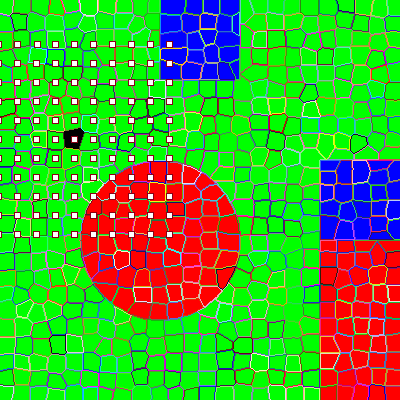
\includegraphics[width=\textwidth]{nonlinear_intro/grid_5.png}
        \caption{grid $11 \times 11$}
      \end{subfigure}
    \caption{Sample grid defining region of influence for a given superpixel.}
    \label{fig:nonlinear_grid}
\end{figure}
Figure \ref{fig:nonlinear_grid} presents two grids, a $7 \times 7$ and $11 \times 11$ grid, that were created for the same sample superpixel in the same image which is marked with a black colour.

Having defined which superpixels have an influence on a superpixel under consideration, it is possible to define its feature vector. The first type of features that were used in the described system are colours of the superpixels from the grid. Those features are discrete, as after the process of colour quantisation only three values are available: red, green, and blue. Hence, taking for example a superpixel from a grid depicted in Figure \ref{fig:grid_7_7}, the contextual colour feature can be expressed as a vector of 49 values, each being a colour of one superpixel. Figure \ref{fig:grid_colour} depicts a visual representation of values from this vector with each feature being shown as a separate coloured box. The feature of a colour of the superpixel under consideration was marked with a pink border.
\begin{figure}[ht]
    \centering
    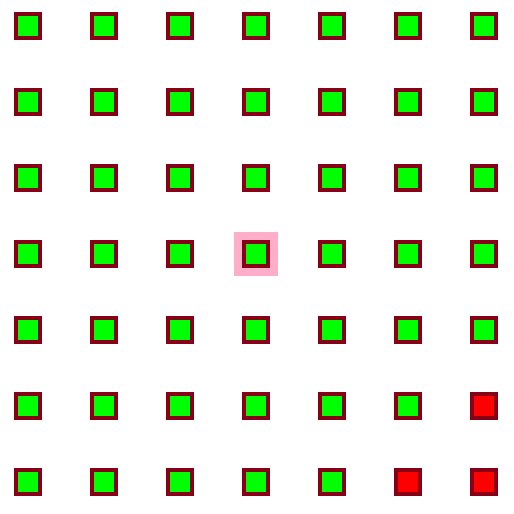
\includegraphics[width=0.55\textwidth]{nonlinear_intro/grid_colour.png}
    \caption{Grid colour features for a sample superpixel.}
    \label{fig:grid_colour}
\end{figure}

The second type of features used in the system was also based on the described grid. However, instead of taking the colour of a superpixel in which a grid point lies, the colours of this superpixel neighbours are taken into consideration. For every superpixel from the grid, the percentage of red, green and blue coloured neighbours is computed. Hence, for a grid $7 \times 7$ there are 49 triplets, which gives all together additional 147 features. Figure \ref{fig:grid_colour_neighbour} serves as an example of how those features are calculated. In this image, values of \nth{121}, \nth{122} and \nth{123} features are to be computed, which are the percentage of red, green and blue neighbours for a superpixel that is marked in pink. 
\begin{center}
    \centering
    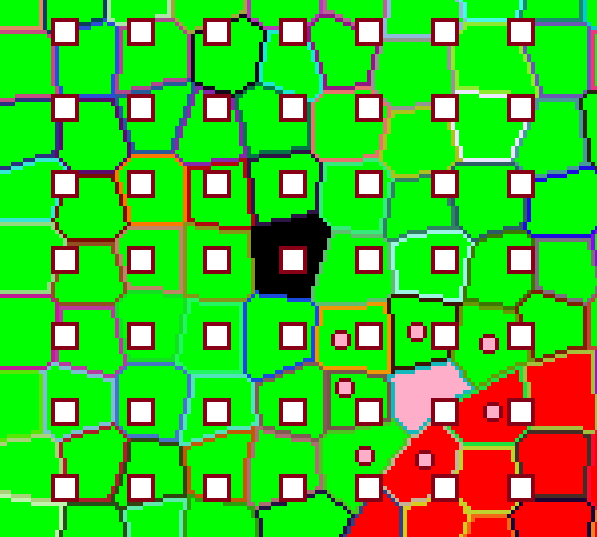
\includegraphics[width=0.55\textwidth]{nonlinear_intro/grid_neighbours.png}
    \captionof{figure}{A sample superpixel from the grid with its closest neighbours marked.}
    \label{fig:grid_colour_neighbour}
\end{center}
The superpixel under consideration has seven closest neighbours, each marked with a pink circle, out of which five are green, two are red, and none are blue. Therefore, value of the \nth{121} feature will be equal to around 0.29, \nth{121} feature will have a value of 0.71, and for \nth{123} feature it will be 0. In such a way, every feature for every superpixel is computed. Similarly, as in the case of the previous type of features, also a visual representation of computed features might be useful especially when comparing two different superpixels. Figure \ref{fig:grid_colour_neighbour_percentage} depicts such a representation. 
\begin{figure}[ht]
    \centering
    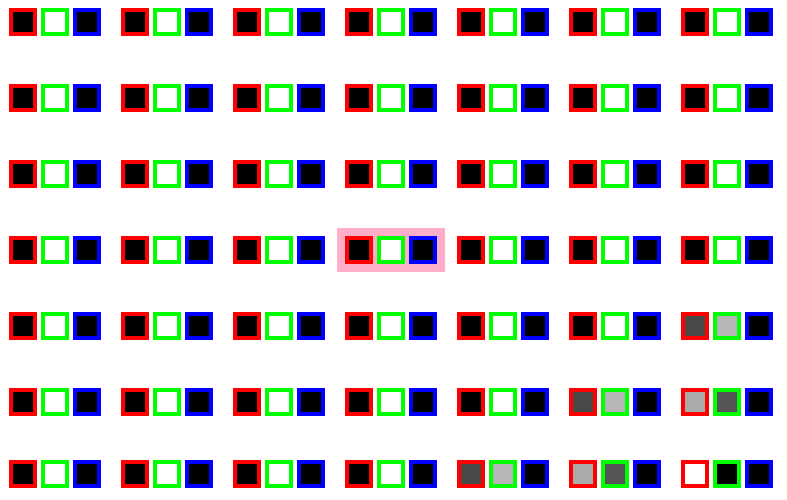
\includegraphics[width=\textwidth]{nonlinear_intro/grid_colour_percentage.png}
    \caption{Grid neighbour colour percentage features for a sample superpixel.}
    \label{fig:grid_colour_neighbour_percentage}
\end{figure}

For each superpixel, three boxes are shown, one per each of the available colours, with a border representing this colour. The percentage of red, green or blue neighbours is expressed as a number between 0 and 1, which is then is multiplied by 255. The inner colour of every box is representing exactly this value. It can be easily seen where there is a boundary between a green and a red region, as the features expressing percentage of green neighbours are gradually changing their colour from all white, meaning 100\% of green neighbours to all black meaning 0\% and conversely a feature for red percentage goes through greyscale colours from black to white. Yet again, features of the superpixels that is under consideration are marked with a pink border.

The presented example was based on the grid $7 \times 7$ in which the percentage of neighbours of the given colour was computed on the closest superpixels only. However, sometimes it might be beneficial to include a larger neighbourhood. Then, instead of processing only adjacent superpixels, also neighbours of those superpixels could be taken into account. The size of this neighbourhood may have a large influence on the results, especially on the borders between two regions. With larger neighbourhood, even if a superpixel has only one neighbour of a different class, this neighbour may be mostly surrounded by superpixels with the same class, and therefore the total percentage of this class may rise. The neighbourhood size is yet another hyperparameter that should be fixed before feature extraction takes place.

With such a definition of features, each superpixel can be defined in terms of a feature vector containing 196 elements. Out of all these features, only such a set should be chosen which carry meaningful information that will allow differentiation of objects by shape. Performing segmentation with too many features is not only more time-consuming, but also less accurate. One of the most popular and simplest algorithms for finding an optimal set of features is a stepwise regression, which was implemented in the thesis. This is a greedy algorithm that creates a resulting set of features step by step. This method can involve only forward steps, only backward steps, or a combination of those two. Forward selection starts by an empty set of features and the first step is to choose such a feature from the whole feature set that will give the highest accuracy of segmentation for a validation set. Then, in each iteration a new best feature is added to the set of already chosen features. Figure \ref{fig:greedy_selection} presents an example of how this method is applied for feature selection from a set of five available features, each depicted as a separate coloured block. Numbers in those blocks represent the accuracy of segmentation for a set of features under consideration. As presented, in the initial iteration a green feature gives the highest accuracy of 62\%, therefore it would be chosen as the first element of the resulting set. Next, the violet feature would be added to a green one as the accuracy of segmentation based on this pair of features is the highest. Similarly, the red and blue features would be added in the following step. In the \nth{5} iteration the segmentation accuracy would drop by adding another feature to a chosen set, therefore in this step the algorithm would stop and the final feature set would be the one chosen in the previous iteration.
\begin{figure}[ht]
    \centering
    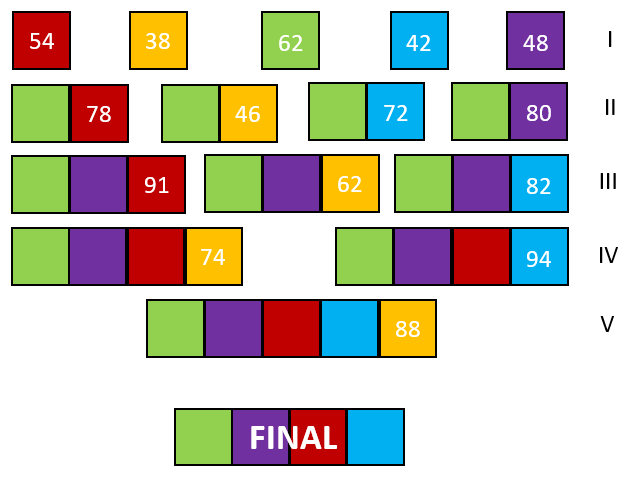
\includegraphics[width=0.75\textwidth]{images/nonlinear_intro/greedy_forward.png}
    \caption{Greedy forward feature selection.}
    \label{fig:greedy_selection}
\end{figure}

In every step, the best feature is added to the chosen set of features, therefore there needs to be a method of assessment based on which feature set the segmentation will give the highest accuracy. As the process of feature selection is applied only to choose features for the unary component of energy, there is no need to perform a full inference process to check the segmentation accuracy. Instead, it is enough to choose the most probable label for each superpixel basing on the computation of unary potential and compare the final labelling to the ground truth, and this is the measure that was implemented to choose the best feature in the current step. Hence, in the first iteration for all sets containing only one element this procedure is performed and the feature with the highest accuracy is added to the final set. Then, to this feature every other feature is added forming sets of two elements and again, the accuracy of segmentation for each set is measured. This procedure continues iteratively until no more features are left, or until a situation in which adding any other feature results in worsening of the model performance. 
Backward feature selection is a very similar process, however, instead of adding new features to the set under consideration, feature elimination is performed. The procedure starts with a full set of available features and then iteratively, the worst feature is removed from this set until further elimination results in poorer accuracy of segmentation. Another possibility is to join those two methods, and make some steps forward and then some steps backwards. 

Next part of the segmentation process that happens after feature selection concerns a feature function definition. Initially, the same feature function was used as in the case of colour-based segmentation, however, the obtained results were really poor. Not only did the method fail to distinguish between red objects of different shapes, but it was also not capable of assigning the proper class to any blue region. Figure \ref{fig:linear_as_nonlinear} presents the results of such segmentation on four sample images. 
\begin{figure}[ht]
    \begin{minipage}{.5\linewidth}
        \begin{tabular}{cc}
            \fcolorbox{black}{white}{\includegraphics[width = 0.41\textwidth]{nonlinear_noise_free/experiments/init/17.png}} &
            \fcolorbox{black}{white}{\includegraphics[width = 0.41\textwidth]{linear_as_nonlinear/17.png}} \\ 
            \fcolorbox{black}{white}{\includegraphics[width = 0.41\textwidth]{nonlinear_noise_free/experiments/init/19.png}} &
            \fcolorbox{black}{white}{\includegraphics[width = 0.41\textwidth]{linear_as_nonlinear/19.png}}
        \end{tabular}
    \end{minipage}%
    \begin{minipage}{.5\linewidth}
        \begin{tabular}{cc}
            \fcolorbox{black}{white}{\includegraphics[width = 0.41\textwidth]{nonlinear_noise_free/experiments/init/20.png}} &
            \fcolorbox{black}{white}{\includegraphics[width = 0.41\textwidth]{linear_as_nonlinear/20.png}} \\ 
            \fcolorbox{black}{white}{\includegraphics[width = 0.41\textwidth]{nonlinear_noise_free/experiments/init/23.png}} &
            \fcolorbox{black}{white}{\includegraphics[width = 0.41\textwidth]{linear_as_nonlinear/23.png}}
        \end{tabular}
    \end{minipage} 
    \caption{Results of shape-based semantic image segmentation using a standard feature function.}
    \label{fig:linear_as_nonlinear}
\end{figure}

As the already implemented feature function did not perform well on the task assigned for this part of the system, a different way of representing features had to be chosen. For the experiments described in this chapter, a feature function for unary potential was expressed as a conditional probability of assigning a label to the current pixel given its features. Then, having an optimal feature vector constructed, it is possible to express unary potential as a negative log-likelihood of a superpixel label given its features as in equation \ref{eq:nonlinear_unary_potential}. 
\begin{equation}
    \label{eq:nonlinear_unary_potential}
    \varphi(x_i,y_i) = -\log p(y_i|f_i)
\end{equation}
In order to compute a probability of a label conditioned on superpixel features, it was necessary to know what is the probability distribution of all labels and all features that were chosen during the process of stepwise regression. Estimation of this distribution is made only once, just after the stage of preprocessing, which divides images into superpixels, and is then used during the training and inference phases to compute the system energy. 